% Giacomo Petrillo
% lezione di Francavilla

\subsection{Esercizi}

\begin{exercise}
	Abbiamo 5 sacchi (grossi) con palline bianche e nere.
	I sacchi hanno frazioni di palline bianche rispettivamente
	\SI1\%, \SI5\%, \SI{50}\%, \SI{95}\%, \SI{99}\%.
	Estraggo da un sacco 5 palline.
	Identificare il sacco con un livello di confidenza del \SI{95}\%.
\end{exercise}

\begin{solution*}
	Sia $m$ la frazione di palline bianche nel sacco
	e $k$ il numero di palline bianche estratte.
	Assegnamo distribuzione binomiale a $k$:
	\begin{equation*}
		p(k;m)
		= \binom 5k m^k (1-m)^{5-k}.
	\end{equation*}
	Costruiamo la banda di confidenza con il probability ordering.
	Innanzitutto tabuliamo $p(k;m)$:
	\begin{center}
		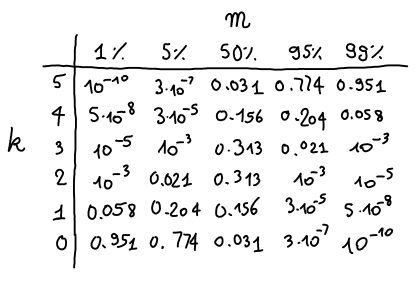
\includegraphics[width=20em]{sacchia}
	\end{center}
	Poi, in ogni colonna,
	aggiungiamo elementi partendo da quello maggiore finché la somma non raggiunge
	il livello di confidenza:
	\begin{center}
		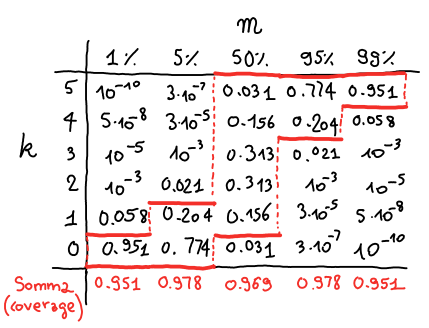
\includegraphics[width=20em]{sacchib}
	\end{center}
	Per $m=\SI{50}\%$ abbiamo scelto arbitrariamente di includere $k=5$ anziché $k=0$.
	Il livello di confidenza effettivamente ottenuto è il minimo dei coverage quindi \SI{95.1}\%.
	Ridisegnamo la banda mettendo in evidenza le stime intervallari ottenute:
	\begin{center}
		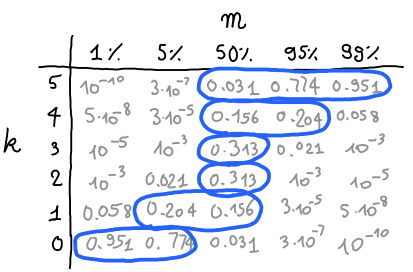
\includegraphics[width=20em]{sacchic}
	\end{center}
\end{solution*}

\begin{exercise}
	\label{th:gausssup}
	Mettere un limite superiore alla media di una gaussiana con varianza fissata.
\end{exercise}

\begin{solution*}
	La distribuzione è
	\begin{equation*}
		p(x;\mu)
		= \frac1{\sqrt{2\pi}\sigma} \exp \left( -\frac12\left(\frac{x-\mu}\sigma\right)^2 \right).
	\end{equation*}
	Definiamo $\phi$ come la cdf della gaussiana con media nulla e varianza unitaria:
	\begin{equation*}
		\phi(y)
		\is \int_{-\infty}^y \de z\, \frac1{\sqrt{2\pi}} e^{-\frac12 z^2},
	\end{equation*}
	la cdf per media $\mu$ e varianza $\sigma$ si ottiene con
	\begin{equation*}
		\phi\left(\frac{x-\mu}\sigma\right).
	\end{equation*}
	Per mettere limiti superiori a $\mu$ scegliamo intervalli per $x$ da $x_\mathrm{min}$ a $\infty$.
	L'equazione per $x_\mathrm{min}$ è
	\begin{align*}
		\mathrm{CL}
		&= 1 - \phi\left(\frac{x_\mathrm{min}-\mu}\sigma\right) \implies \\
		\implies \frac{x_\mathrm{min}-\mu}\sigma
		&= \phi^{-1}(1-\mathrm{CL}) = -\phi^{-1}(\mathrm{CL}) \implies \\
		\implies x_\mathrm{min}
		&= \mu - \sigma\phi^{-1}(\mathrm{CL}),
	\end{align*}
	da cui otteniamo
	\begin{equation*}
		\mu_\mathrm{max} = x + \sigma\phi^{-1}(\mathrm{CL}).
	\end{equation*}
\end{solution*}

\begin{exercise}
	Ripetere l'\autoref{th:gausssup} con limite inferiore, probability ordering e likelihood ratio.
\end{exercise}

\begin{solution}
	Per il limite inferiore si ottiene
	\begin{equation*}
		\mu_\mathrm{min}
		= x - \sigma\phi^{-1}(\mathrm{CL}),
	\end{equation*}
	con il probability ordering si ottiene l'intervallo delimitato da
	\begin{equation*}
		x \pm \sigma\phi^{-1} \left( 1- \frac{1-\mathrm{CL}}2 \right).
	\end{equation*}
	Poiché
	\begin{equation*}
		\sup\limits_\mu p(x;\mu)
		= \frac1{\sqrt{2\pi}\sigma}
	\end{equation*}
	non dipende da $x$,
	il likelihood ratio è equivalente al probability ordering.
\end{solution}

\begin{exercise}
	Ripetere l'\autoref{th:gausssup} con likelihood ratio e dominio $\mu>0$.
\end{exercise}

\begin{solution*}
	Fissiamo $\sigma=1$.
	Calcoliamo il likelihood ratio:
	\begin{align*}
		\sup\limits_{\mu>0} p(x;\mu)
		&= \begin{cases}
			p(x;x) & x \ge 0 \\
			p(x;0) & x < 0
		\end{cases} = \\
		&= \frac1{\sqrt{2\pi}} \begin{cases}
			1                & x \ge 0 \\
			e^{-\frac12 x^2} & x < 0,
		\end{cases} \\
		\lambda_\mu(x\ge 0)
		&= 2\log \frac 1 {e^{-\frac12(x-\mu)^2}} = \\
		&= (x-\mu)^2, \\
		\lambda_\mu(x<0)
		&= 2\log \frac {e^{-\frac12 x^2}} {e^{-\frac12 (x^2 - 2\mu x + \mu^2)}} = \\
		&= -2\mu x + \mu^2.
	\end{align*}
	La funzione di ordinamento è infine
	\begin{equation*}
		O(\mu,x)
		= \begin{cases}
			- (x-\mu)^2 & x \ge 0 \\
			2\mu x - \mu^2 & x < 0.
		\end{cases}
	\end{equation*}
	Evitiamo di fare i conti per ricavare la banda di confidenza.
\end{solution*}

\begin{exercise}
	Mettere limiti superiori alla media della poissoniana.
\end{exercise}

\begin{solution}
	Bisogna risolvere numericamente l'equazione
	\begin{equation*}
		\mathrm{CL}
		= e^{-\mu} \sum_{k=k_\mathrm{min}}^\infty \frac{\mu^k}{k!}
	\end{equation*}
	per trovare $k_\mathrm{min}(\mu)$ e poi trovare numericamente
	\begin{equation*}
		\mu_\mathrm{max}(k)
		= \max \{\mu \,|\, k=k_\mathrm{min}(\mu)\}.
	\end{equation*}
	Questo è uno script python che esegue i calcoli:
	\lstset{%
		basicstyle=\small,
		numbers=left,
		% keywordstyle=\bfseries\sffamily,
		commentstyle=\rmfamily,
		columns=fullflexible,
		literate=
		  {á}{{\'a}}1 {é}{{\'e}}1 {í}{{\'i}}1 {ó}{{\'o}}1 {ú}{{\'u}}1
		  {Á}{{\'A}}1 {É}{{\'E}}1 {Í}{{\'I}}1 {Ó}{{\'O}}1 {Ú}{{\'U}}1
		  {à}{{\`a}}1 {è}{{\`e~}}1 {ì}{{\`i}}1 {ò}{{\`o}}1 {ù}{{\`u}}1
		  {À}{{\`A}}1 {È}{{\'E}}1 {Ì}{{\`I}}1 {Ò}{{\`O}}1 {Ù}{{\`U}}1
		  {ä}{{\"a}}1 {ë}{{\"e}}1 {ï}{{\"i}}1 {ö}{{\"o}}1 {ü}{{\"u}}1
		  {Ä}{{\"A}}1 {Ë}{{\"E}}1 {Ï}{{\"I}}1 {Ö}{{\"O}}1 {Ü}{{\"U}}1
		  {â}{{\^a}}1 {ê}{{\^e}}1 {î}{{\^i}}1 {ô}{{\^o}}1 {û}{{\^u}}1
		  {Â}{{\^A}}1 {Ê}{{\^E}}1 {Î}{{\^I}}1 {Ô}{{\^O}}1 {Û}{{\^U}}1
		  {œ}{{\oe}}1 {Œ}{{\OE}}1 {æ}{{\ae}}1 {Æ}{{\AE}}1 {ß}{{\ss}}1
		  {ű}{{\H{u}}}1 {Ű}{{\H{U}}}1 {ő}{{\H{o}}}1 {Ő}{{\H{O}}}1
		  {ç}{{\c c}}1 {Ç}{{\c C}}1 {ø}{{\o}}1 {å}{{\r a}}1 {Å}{{\r A}}1
		  {€}{{\euro}}1 {£}{{\pounds}}1 {«}{{\guillemotleft}}1
		  {»}{{\guillemotright}}1 {ñ}{{\~n}}1 {Ñ}{{\~N}}1 {¿}{{?`}}1
	}
	\lstinputlisting[language=Python]{../poissonsup.py}
\end{solution}

\begin{exercise}
	Banda di confidenza per $p$ della binomiale.
\end{exercise}
